\subsection{Model View Controller(MVC)}
In the web service component of the project we use the ASP.net MVC framework. 
This framework is using the MVC architecture pattern for structuring the code.
This pattern will be described shortly in the following, based on the overview article on the Microsoft website \citet{aspmvc}.

MVC or Model View Controller is used to separate responsibility of an application into three parts, the model, the view, and the controller.
The pattern can be seen as an architecture diagram on \cref{mvcdiagram}.

\begin{figure}[h]
\center
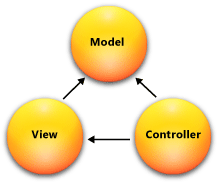
\includegraphics[width=0.4\textwidth]{graphics/mvc}
\caption{The MVC design pattern. From \citet{aspmvc}}
\label{mvcdiagram}
\end{figure}

\begin{itemize}
\item[\textbf{Model}] The model contains the model of the application domain and takes care of fetching data and making them available through the model.
\item[\textbf{View}] View displays the model to the user.
\item[\textbf{Controller}] The controllers handle the interaction with users. Based on userinput the controller works on the model and selects what the view needs to be used for displaying the data.
\end{itemize}